% !TeX root = report.tex
\documentclass[a4paper, 11pt]{article}

%------------------------------------------------------------------------------------
% import packages
\usepackage[scaled]{helvet}
\usepackage{courier}
\renewcommand\familydefault{\sfdefault} 
\usepackage[T1]{fontenc}
\usepackage[english]{babel}
\usepackage{graphicx}
\usepackage{tabularx}
\usepackage{ltablex}
\usepackage{multirow}
\usepackage{caption, booktabs}
\usepackage[hidelinks]{hyperref}
\usepackage[shortlabels]{enumitem}

% Font weight for pictures labels
\usepackage[labelfont=bf]{caption}

% Margins
\usepackage[margin=1in]{geometry}

% Set TOC Depth
\setcounter{tocdepth}{3}

\begin{document}

\begin{titlepage}
	\centering
    \begin{tabular}{rl}
        Alessio Hu & (10683050) \\
        Andrea Franchini & (10560276) \\ 
        Carlo L. Reinotti & (10840446) \\
        Fabio Camerota & (10864017) \\
    \end{tabular}

    \vspace{1.5cm}
    {\Huge \textbf{Usability Evaluation\\}}
    \vspace{1.5cm}
    {\large 
        Hypermedia Applications (Web and Multimedia) \\
        Prof. Garzotto Franca \\ 
		DEIB - Politecnico di Milano \par
    }
    \vspace{1.5cm}
    {\large \textbf{Analyzed website:}\\
    \vspace{0.5cm}
    https://www.yesmilano.it/en}
    \par
    \vspace{3cm}
    
\includegraphics[scale=0.4]{images/logo.pdf}
    \par
    \vspace{3cm}
	A.Y. 2021-2022
    
	
\end{titlepage}

\tableofcontents
    % !TeX root = ../report.tex

\begin{abstract}
    The purpose of this Usability Report is to analyze the results of the usability evaluation of the website ``https://www.yesmilano.it/en'' through two different methods: \emph{inspection} (performed by the group members) and \emph{user testing} (performed by a third party voluntaries belonging to a specific user profile).

    For the inspection, we listed the main functionalities of the website and propose several tasks around them. For each task, we analyzed the website according to Nielsen's and MiLe heuristics, assigning scores and documenting with screenshots the website issues.
    
    For the user testing, we collected data directly from 20 possible final users among two different user profiles (students and tourists). Inspectors asked each user to perform a series of tasks. During the process, the inspector monitored and collected data, following quantitative and qualitative indicators. The collected information is then organized in tables and charts.
    
    The results of the two different methodologies were then combined and final conclusions about the usability properties of the website are explained, furthermore providing some potential fixes and improvements to enhance the user experience while browsing the website.
\end{abstract}

\vspace*{5em}
\section*{Disclaimer}

Since the analyzed website presents many sections, we selected a subset of those; in particular, we analyzed pages belonging to:
\begin{itemize}
    \item Guide to the City
    \item Study
    \item Events
    \item Traveller Information
    \item YesMilano Hotels
    \item YesMilano Restaurants
\end{itemize}

On the other hand, we decided to not consider the following sections:
\begin{itemize}
    \item Invest \& Start up
    \item Convetion Bureau
\end{itemize}
    % !TeX root = ../report.tex

% Key information to be included:
% - Few lines about the general method and the steps followed
% - Heuristics (report the definitions in the previous slides)
% - Metrics agreed among all evaluators
% - Final scores agreed among all evaluators (include the main comments
% for your scores and examples of commentedscreenshots to support
% your scores)
% - Annex: Report the scores and main comments of EACH evaluator
% - PROVIDE AGGREGATED DATA, e.g., MEAN VALUES FOR ALL EURISTICS,
% (MEAN) SCORE BY DIMENSIONS (e.g., for CONTENT HEURISTICS,
% NAVIGATION HEURISTICS, ect.)
% - PROVIDE VISUAL REPRESENTATIONS OF RESULTS (diagrams, summary
% tables...)
% - Include a short conclusion section where you breifly discuss inspection
% results

\section{Inspection}

\subsection{Method}
% what is inspection based usability evaluation
% specific heuristics and metrics used
Inspection-based usability evaluation allows teams of evaluators to perform
a systemic analisys of UI/UX aspects of an application (a website, in our case).
We adopted the widely used \emph{heuristic evaluation}, as the main usability inspection method, in which the evaluators concentrate on a set of principles (``heuristics'') to test the usability of the application.

\subsubsection{Heuristics}

This section explains the different heuristics we adopted to evaluate the
website compliance to usability quality principles. In particular, we used
\emph{Nielsen's} and a subset of \emph{MiLE} (Milano Lugano usability Evaluation method) heuristics.

\paragraph*{Nielsen's heuristics}

\begin{enumerate}[start=1,label={\bf H\arabic{*}}]
    \item \textbf{Visibility of system status:} does the user know where they are and    
          what's going on?
    \item \textbf{Match between system and the real world:} does the system use 
          conventions known to the users?
    \item \textbf{User control and freedom:} can the user leave unwanted state quickly? 
          Is undo/redo available to them?
    \item \textbf{Consistency and standards:} do multiple words/elements/actions mean    
          the same thing?
    \item \textbf{Error prevention:} do the application try to prevent problems 
          from occurring (e.g.: checking inputs before submitting them)?
    \item \textbf{Recognition rather than recall:} are options visible or easily 
          retrievable?
    \item \textbf{Flexibility and efficiency of use:} are accelerators available?
    \item \textbf{Aesthetic and minimalist design:} is dialogue containing only relevant 
          informations?
    \item \textbf{Help users recognize, diagnose and recover from errors:} are error 
          codes in plain language? Do they suggest a possible solution?
    \item \textbf{Help and documentation:} (if any) is it easily searchable?
\end{enumerate}

\paragraph*{MiLE heuristics}

We can further subdivide MiLE heuristics in 3 categories: navigation, content, presentation.

\subparagraph*{Navigation}

\begin{enumerate}[start=1,label={\bf MN\arabic{*}}]
    \item \textbf{Interaction consistency:} do pages of the same type have the same links
          and interaction capability?
    \item \textbf{Group navigation:} is it easy to navigate from and among groups of
          ``items''?
    \item \textbf{Structural Navigation:} is it easy to navigate among the ``components'' of a topic?
    \item \textbf{Semantic Navigation:} is it easy to navigate between related topics?
    \item \textbf{Landmarks:} are landmarks useful to reach the key parts of the web
          site?
\end{enumerate}

\subparagraph*{Content}

\begin{enumerate}[start=1,label={\bf MC\arabic{*}}]
    \item \textbf{Information overload:} is the information in a page too much/too
          little?
\end{enumerate}

\subparagraph*{Presentation}

\begin{enumerate}[start=1,label={\bf MP\arabic{*}}]
    \item \textbf{Text lay out:} is the text readable? Is font size appropriate?
    \item \textbf{Interaction placeholders-semiotics:} are textual or visual    
          labels of interactive elements ``expressive'' and meaningful?
    \item \textbf{Interaction placeholders-consistency:} are textual or visual 
          labels of interactive elements consistent in terms of wording, icon, 
          position, etc.?
    \item \textbf{Spatial allocation:} is the on-screen allocation of contents 
          and visual appropriate for their relevance? Are ``semantically 
          related'' elements close and ``semantically distant'' element far 
          away?
    \item \textbf{Consistency of Page Structure:} do pages of the same type 
          have the same layout?
\end{enumerate}

\subsubsection{Metrics}

To keep the inspection process straightforward, we agreed on evaluating the compliance of the website to each heuristic on a scale from 0 to 3, without decimals. In this way, we avoid situations where it's hard to define the difference two close numbers on larger scales (e.g.: 6 and 7 on a scale from 1 to 10).

\begin{figure*}[h]
    \begin{tabular}{c l l}
        \toprule
        \textbf{Score} & \textbf{Meaning} & \textbf{Comment} \\
        \midrule
        0 & Bad & Heuristic not satified at all \\
        1 & Worse than better & There are multiple violations of the heuristic \\
        2 & Better than worse & Overall the heuristic is satified with some  exception \\
        3 & Good & Heuristic satified\\
        \bottomrule
    \end{tabular}
\end{figure*}

Since not all heuristics apply in all situations, we could also assign a ``N/A'' (``not applicable'') in such cases.

\subsection{Execution of the study}
% How the study was performed

\subsection{Results}
Inspection was initially carried out individually by each evaluator. At the end of this first phase, a meeting was held in order to reach an agreed score for each heuristic. The final scores agreed on usually differed from the arithmetic mean: the level of disagreement over each topic (represented by the variance) was also considered.
Graphical results are represented in Fig \ref{BarsNielsenCrop} and in Fig \ref{BarsMileCrop}.

\begin{figure}[!ht]
    \begin{minipage}{\linewidth}
        \centering
        \makebox[\textwidth][c]{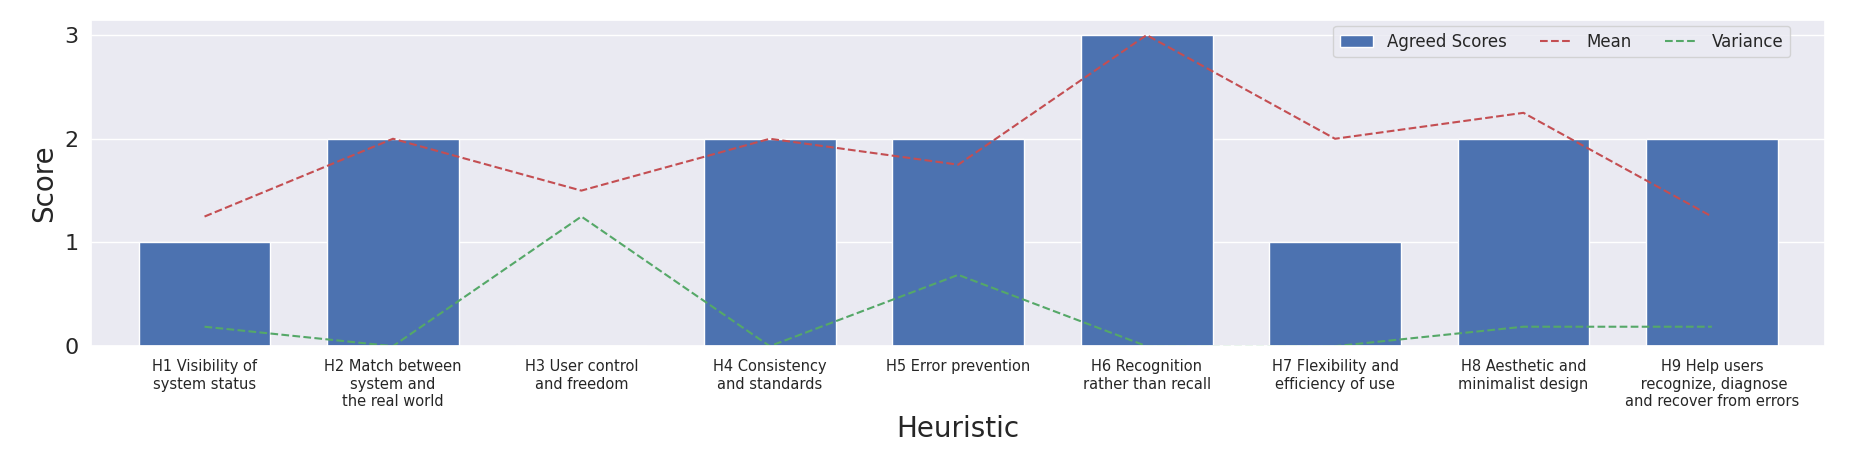
\includegraphics[width=1.2\textwidth]{images/BarsNielsenCrop.png}}%
        \captionsetup{justification=centering}
        \caption{Nielsen heuristics evaluation summary}
        \label{BarsNielsenCrop}
    \end{minipage}
\end{figure}

\begin{figure}[!ht]
    \begin{minipage}{\linewidth}
        \centering
        \makebox[\textwidth][c]{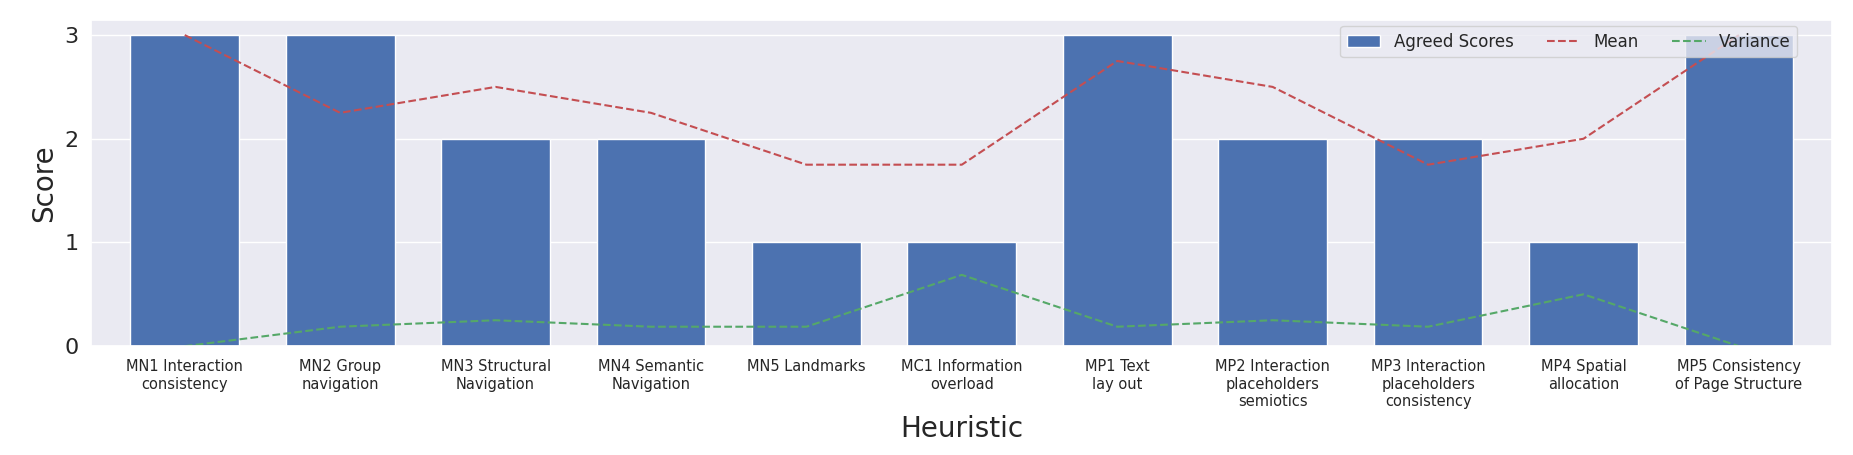
\includegraphics[width=1.2\textwidth]{images/BarsMileCrop.png}}%
        \captionsetup{justification=centering}
        \caption{Mile heuristics evaluation summary}
        \label{BarsMileCrop}
    \end{minipage}
\end{figure}

\begin{tabularx}{\linewidth}{l c X}
\toprule
\textbf{Heuristic} & \textbf{Score} & \textbf{Comment} \\
\midrule
\endfirsthead
\toprule
\textbf{Heuristic} & \textbf{Score} & \textbf{Comment} \\
\midrule
\endhead
\midrule
\footnotesize [Continues on next page]
\endfoot
\bottomrule
\endlastfoot
    % body
    H1 & 1 & There is a difficulty in navigation as breadcrumbs are sometimes either missing or incorrect.\par When using the search bar, there is no feedback on the progress status, the page can appear frozen. \\ \midrule
    H2 &  & \\ \midrule
    H3 &  & \\ \midrule
    H4 &  & \\ \midrule
    H5 &  & \\ \midrule
    H6 &  & \\ \midrule
    H7 &  & \\ \midrule
    H8 &  & \\ \midrule
    H9 &  & \\ \midrule
    H10 &  &
\end{tabularx}

\paragraph{Mile}


\begin{tabularx}{\linewidth}{l c c X}
\toprule
\textbf{Category} & \textbf{Heuristic} & \textbf{Score} & \textbf{Comment} \\
\midrule
\endfirsthead
\toprule
\textbf{Category} & \textbf{Heuristic} & \textbf{Score} & \textbf{Comment} \\
\midrule
\endhead
\midrule
\footnotesize [Continues on next page]
\endfoot
\bottomrule
\endlastfoot

\multirow{5}{*}{\textbf{Navigation}}   & MN1 & 0 & Lorem ipsum Lorem ipsum Lorem ipsum Lorem ipsum Lorem ipsum \\ \cmidrule{2-4} 
                                        & MN2 &  &  \\ \cmidrule{2-4} 
                                        & MN3 &  &  \\ \cmidrule{2-4} 
                                        & MN4 &  &  \\ \cmidrule{2-4} 
                                        & MN5 &  &  \\ \midrule
\textbf{Content}                       & MC1 &  &  \\ \midrule
\multirow{5}{*}{\textbf{Presentation}} & MP1 & 3 & The text is always readable and of the appropriate size \\ \cmidrule{2-4} 
                                        & MP2 & 2 & Some labels and and icons are not expressive enough and do not reflect the meaning of the interaction and its effects\\ \cmidrule{2-4} 
                                        & MP3 & & \\ \cmidrule{2-4} 
                                        & MP4 &  &  \\ \cmidrule{2-4} 
                                        & MP5 &  &
\end{tabularx}

bla bl
\subsection{Discussion of results}
\subsubsection{Discussion within Nielsen's heuristics}
\begin{itemize}
    \item \textbf{H1 Visibility of system status}\\
    Commento su heuristic (Figura \ref{fig:1-image-ref})
    \begin{figure}[!ht]
        \begin{minipage}{\linewidth}
            \centering
            \captionsetup{justification=centering}
            \makebox[\textwidth][c]{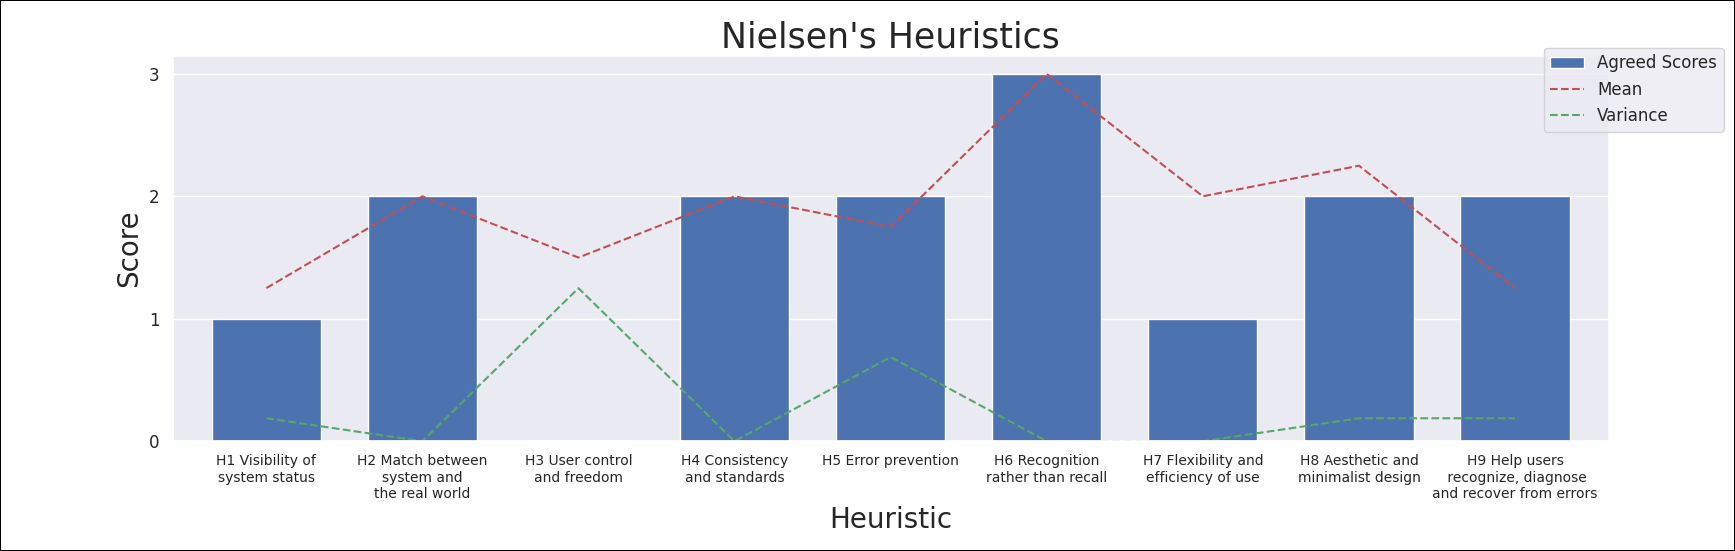
\includegraphics[width=0.7\textwidth]{images/test.png}}%
            \caption{Label dell'immagine}
            \label{fig:1-image-ref}
        \end{minipage}
    \end{figure}
    \item \textbf{Nielsen 2}\\
    Bla bla
    \item bla bla
\end{itemize}

\subsubsection{Discussion within Mile's heuristics}
\begin{itemize}
    \item \textbf{MP1 Text lay out}\\
    No critical aspects found, the text is always readable and of the appropriate size.\\
    \item \textbf{MP2 Interaction placeholders-semiotics}\\
    A few minor problems were found in this heuristic: some icons are mismatched with regards to their meaning, and there are labels that are unclear in their functionalities (Fig. \ref{MP2-1} and \ref{MP2-2})
    \begin{figure}[!ht]
        \begin{minipage}{\linewidth}
            \centering
            \makebox[\textwidth][c]{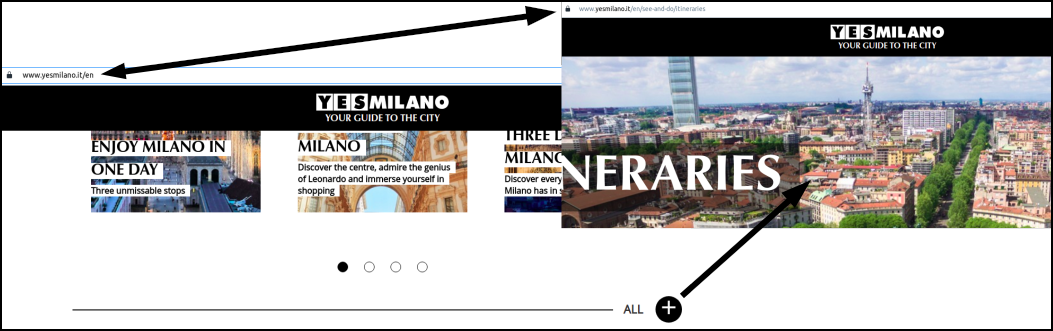
\includegraphics[width=1.2\textwidth]{images/MP2-1.png}}%
            \captionsetup{justification=centering}
            \caption{Conventionally, the "+" should expand the page,\\but in this case the button leads to a new page}
            \label{MP2-1}
        \end{minipage}
    \end{figure}
    \begin{figure}[!ht]
        \begin{minipage}{\linewidth}
            \centering
            \makebox[\textwidth][c]{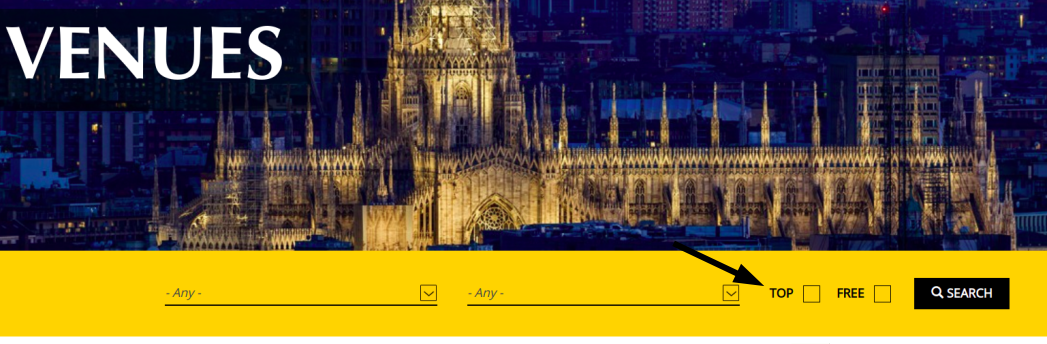
\includegraphics[width=1\textwidth]{images/MP2-2.png}}%
            \captionsetup{justification=centering}
            \caption{In the venues form page, it's unclear what does "TOP" mean in this context.\\If it's based on users reviews, there is no rating system explained}
            \label{MP2-2}
        \end{minipage}
    \end{figure}
\end{itemize}

\pagebreak
Commento
    % !TeX root = ../report.tex

\section{User Testing}
\subsection{Method}
%General method (what is UT)
%Copy and past of definition

User Testing is a methodology aimed at evaluating the usability of an application, where by "usability" we mean "the effectiveness, efficiency and satisfaction with which specified users can achieve specified goals in particular environments" (ISO 9241-11). Therefore, User Testing is a task-oriented empirical research which involves end users that are observed by researchers while the former are using the application.

\subsection{Design of the study}
    The user testing was performed both remotely and in-presence, with the use of two personal computers, one for the end user and one for the evaluator. 
    
    In case of an remote approach, the users were asked to share their screen via a videoconferencing software to let the evaluator observe their actions.

    \subsubsection{User profile and recruitment}
    % Explain the two different user profiles
    For our analysis, we selected two User Profiles:

    \begin{itemize}
        \item College students that live in Milan 
        \item Tourists that wants to visit the city
    \end{itemize}

    Both the user profiles were selected between the age of 20 and 30 years old.

    For the recruitment, each evaluator has recruited 5 users between friends or relatives of the evaluator.

    \subsubsection{Metrics and indicators}
    \paragraph{Quantitative and qualitative indicators}
    Both quantitative and qualitative indicators were measured. 
    
    The quantitative indicators were:
    \begin{itemize}
        \item Effectiveness (task success rate)
        \item Efficiency (time on task)
        \item Errors (wrong paths or actions)
        \item Perceived tasks difficulty
    \end{itemize}

    Such indicators were measured by assigning a score to each of them while the users were performing the tasks. Whereas for qualitative indicators, we collected short textual descriptions of how the user was performing during the task.

    \paragraph{Scoring}
    The effectiveness was measured using this scoring method:
    \begin{itemize}
        \item 1 point if the user has successfully completed the task, without requiring any assistance;
        \item 0.5 points if the user was able to complete the task, but requesting the examiner's assistance for one or more steps;
        \item 0 points if the user has given up, or has thought he has finished when he has not.
    \end{itemize}

    The efficiency was measured by the time (in minutes and seconds) taken by the user to complete the task.\\
    The number of errors is the number of wrong paths or actions taken by the user while completing the task.\\
    The perceived tasks difficulty was measured by asking the user to assign a score from 1 (very easy)  to 5 (impossible).

    \subsubsection{Tasks}
    % Tasks list
    % Explain that for each different user profile different task
    We have defined 6 tasks per user profile, so as to further analyze the most relevant sections of the site that we had already inspected in the inspection phase.

    Although the tasks assigned to each user profile have been defined according to the importance for the specific user, some tasks overlap because they are interesting for both user profiles.

    The site has both simple and complex features so we have defined both simple and complex tasks, to simulate the experience of a real user.
    
    For the user profile ``college students that live in Milan'' we defined the following tasks:

    \begin{enumerate}
        
        \item You are a design student at polimi. You want to see what are the major art events of the year, in particular look for the triennale.
        \item You are considering which university to enroll to. Try to find out which are the universities in Milan that offer a bachelor degree in economics as an Exchange/International Student.
        \item You are an exchange student from US, and you will rent a house here at Milan. Find the required documents to sign a tenancy contract.
        \item You want to move around and orient yourself in Milan. Find information and download the map about public transports.
        \item You are interested in visiting Milano, but you are unsure of the covid situation of the city and its policies (e.g. regarding green pass). Find more about it and where to get tested.
        \item You want to find the list of museums in Milano whose entrance is free. Select the first and look for its opening times, how to reach it and if there are any parking spots. 
    \end{enumerate}
        For the user profile "tourists that wants to visit the city" we defined the following tasks:
    \begin{enumerate}
        \item For this saturday, you've planned to shop at Porta Venezia till lunch time. Find and book the nearest restaurant in the area for that saturday, in particular you are a vegan.
        \item You are planning to book an hotel near the city center (Duomo) for the weekend for two adults, a child and your lovely dog.
        \item You are a tourist with three free days, search a suitable itinerary in Milan that may last from one up to three days.
        \item You want to move around and orient yourself in Milan. Find information and download the map about public transports.
        \item You are interested in visiting Milano, but you are unsure of the COVID situation in the city and its policies (e.g. regarding the green pass). Find more about it and where to get tested.
        \item You want to find the list of museums in Milano whose entrance is free. Select the first and look for its opening times, how to reach it and if there are any parking spots.
    \end{enumerate}
    
\subsection{Execution of the study}
    % Explain that each inspector had 5 users, 3 students and 2 tourists (or viceversa)
    % Timer, in presence and in remote interview
    % Google form, can include some screenshots
    (unire tale parte con "Design of the study"???)\\
    As stated above, each inspector has recruited 5 users. In particular, two of us have recruited 3 students and 2 tourists and the other two have recruited 2 students and 3 tourists. So we have a total of 20 users, including 10 students and 10 tourists.\\
    To easily collect the data we used a Google Form, the results of which were automatically uploaded to an Excel file. This greatly simplified the process of analysing the results.\\
    To avoid similar results for each tasks and a learning factor which would always penalize the performance of the very first task assigned to an user, we randomized the order of execution of the tasks.

\subsection{Results}
    % Final scores (with comments);
    % Aggregates scores (with visualizations)

    We distinguish each user through an ID composed of the type of the profile, the evaluator name and a numerical value, for example S-1-Alessio identifies the very first student interviewed by Alessio. We also identify the various tasks through and ID composed of the type of the profile and a number.
\subsubsection{Effectiveness}
    The table below shows the success rate for each user for each task, following the scoring method mentioned before. Blank cells mean that the user was not given that specific task to do as it was not coherent with the user's profile.\\
    The last row of the table shows the aggregate completion percentage for each task.
    % Effectiveness
    %   - table
    \begin{tabularx}{\linewidth}{l|c|c|c|c|c|c|c|c|c}
    \toprule
    \textbf{User ID} & \textbf{S1} & \textbf{S2} & \textbf{S3} & \textbf{T1} & \textbf{T2} & \textbf{T3} & \textbf{S4-T4} & \textbf{S5-T5} & \textbf{S6-T6} \\
    \midrule
    \endfirsthead
    \toprule
    \textbf{User ID} & \textbf{S1} & \textbf{S2} & \textbf{S3} & \textbf{T1} & \textbf{T2} & \textbf{T3} & \textbf{S4-T4} & \textbf{S5-T5} & \textbf{S5-T5} \\
    \midrule
    \endhead
    \midrule
    \footnotesize [Continues on next page]
    \endfoot
    \bottomrule
    \endlastfoot
        % body
        S-Alessio-1 & 1 & 1 & 1 &  &  &  & 1 & 1 & 0.5 \\ \midrule
        S-Alessio-2 & 1 & 1 & 1 &  &  &  & 1 & 1 & 0 \\ \midrule
        S-Alessio-3 & 0.5 & 1 & 1 &  &  &  & 1 & 1 & 0.5 \\ \midrule
        S-Andrea-1 & 0.5 & 0.5 & 1 &  &  &  & 1 & 1 & 0.5 \\ \midrule
        S-Andrea-3 & 1 & 1 & 1 &  &  &  & 1 & 1 & 0 \\ \midrule
        S-Andrea-5 & 1 & 1 & 1 &  &  &  & 0.5 & 1 & 0.5 \\ \midrule
        S-Carlo-2 & 0.5 & 1 & 1 &  &  &  & 1 & 1 & 0 \\ \midrule
        S-Carlo-4 & 1 & 1 & 0 &  &  &  & 1 & 1 & 1 \\ \midrule
        S-Fabio-1 & 0 & 1 & 0.5 &  &  &  & 1 & 1 & 0 \\ \midrule
        S-Fabio-2 & 1 & 1 & 1 &  &  &  & 1 & 1 & 0 \\ \midrule
        T-Alessio-4 &  &  &  & 0 & 1 & 0.5 & 1 & 1 & 1 \\ \midrule
        T-Alessio-5 &  &  &  & 1 & 1 & 1 & 1 & 1 & 0 \\ \midrule
        T-Andrea-2 &  &  &  & 1 & 1 & 0 & 1 & 1 & 1 \\ \midrule
        T-Andrea-4 &  &  &  & 0.5 & 0.5 & 1 & 1 & 1 & 0.5 \\ \midrule
        T-Carlo-1 &  &  &  & 1 & 1 & 1 & 1 & 1 & 0.5 \\ \midrule
        T-Carlo-3 &  &  &  & 1 & 0.5 & 1 & 1 & 1 & 0.5 \\ \midrule
        T-Carlo-5 &  &  &  & 1 & 1 & 1 & 1 & 1 & 1 \\ \midrule
        T-Fabio-3 &  &  &  & 1 & 1 & 1 & 1 & 1 & 0.5 \\ \midrule
        T-Fabio-4 &  &  &  & 0.5 & 1 & 1 & 1 & 1 & 0.5 \\ \midrule
        T-Fabio-5 &  &  &  & 1 & 1 & 1 & 1 & 1 & 0 \\ \midrule
        \textbf{Completion Rate} & \textbf{75\%} & \textbf{95\%} & \textbf{85\%} & \textbf{80\%} & \textbf{90\%} & \textbf{85\%} & \textbf{97\%} & \textbf{100\%} & \textbf{42\%}
    \end{tabularx}

\subsubsection{Efficiency}
    % Efficiency
    %   - table
    %   - Bar chart with (tasks, avg of completion time) for each dataset
    The evaluator measured the time spent on each task from each user. A graphical representation of all the measured times is provided in Fig. \ref{ResultsEfficiencyStudent} and in Fig. \ref{ResultsEfficiencyTourist}. We remind that the order of execution of the tasks is random and differs for each user, in the graphs the bars are shown in order for simplicity.\\
    An additional bar graph in Fig. \ref{ResultsEfficiencyAvg} represents the average completion time per task.

    \begin{figure}[!ht]
        \begin{minipage}{\linewidth}
            \centering
            \makebox[\textwidth][c]{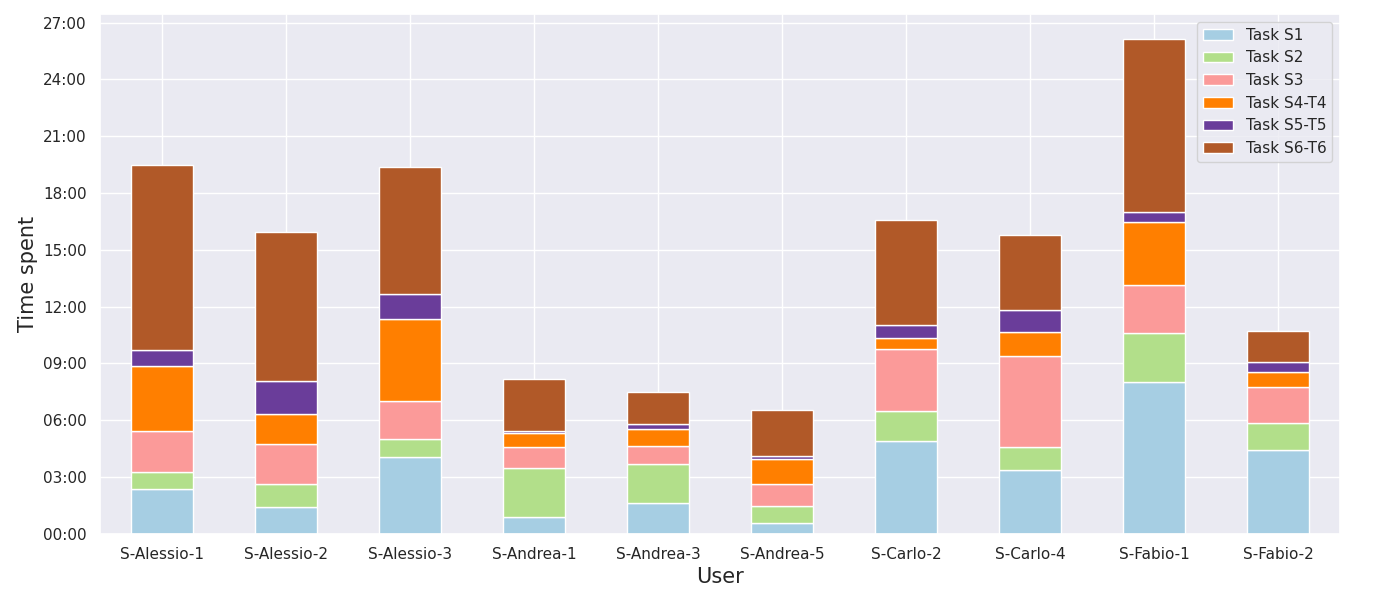
\includegraphics[width=1\textwidth]{images/ResultsEfficiencyStudent.png}}%
            \captionsetup{justification=centering}
            \caption{Time spent on each task for each student}
            \label{ResultsEfficiencyStudent}
        \end{minipage}
    \end{figure}
    \begin{figure}[!ht]
        \begin{minipage}{\linewidth}
            \centering
            \makebox[\textwidth][c]{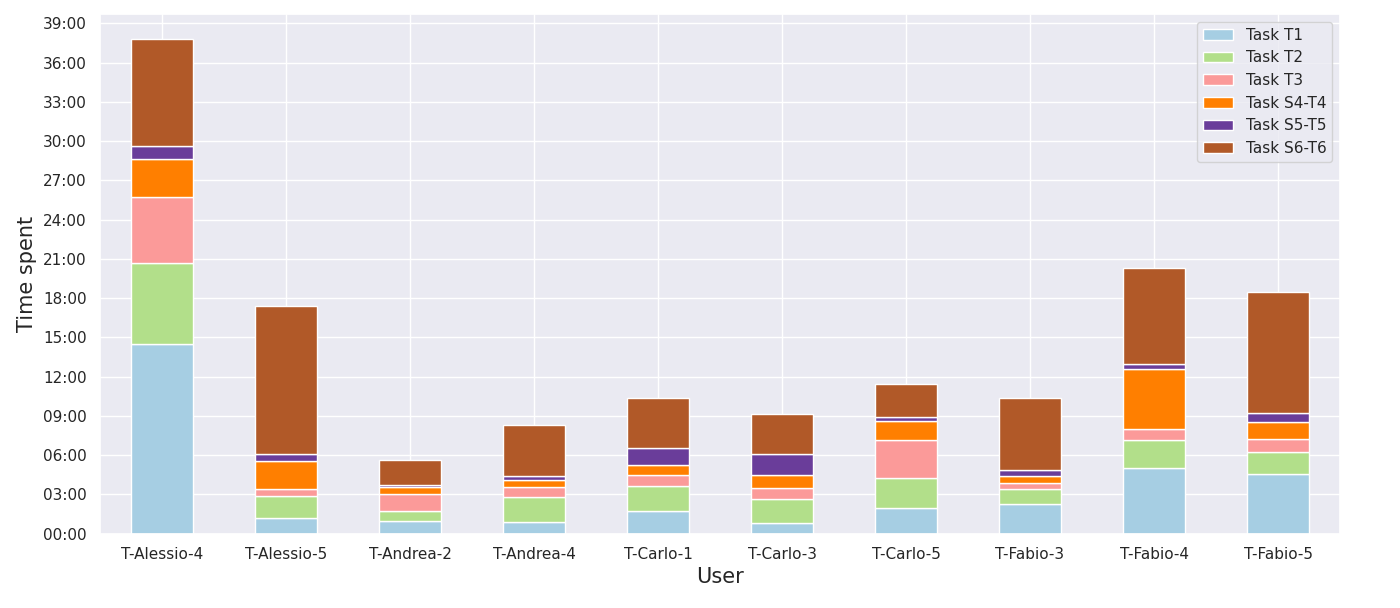
\includegraphics[width=1\textwidth]{images/ResultsEfficiencyTourist.png}}%
            \captionsetup{justification=centering}
            \caption{Time spent on each task for each tourist}
            \label{ResultsEfficiencyTourist}
        \end{minipage}
    \end{figure}


    \begin{figure}[!ht]
        \begin{minipage}{\linewidth}
            \centering
            \makebox[\textwidth][c]{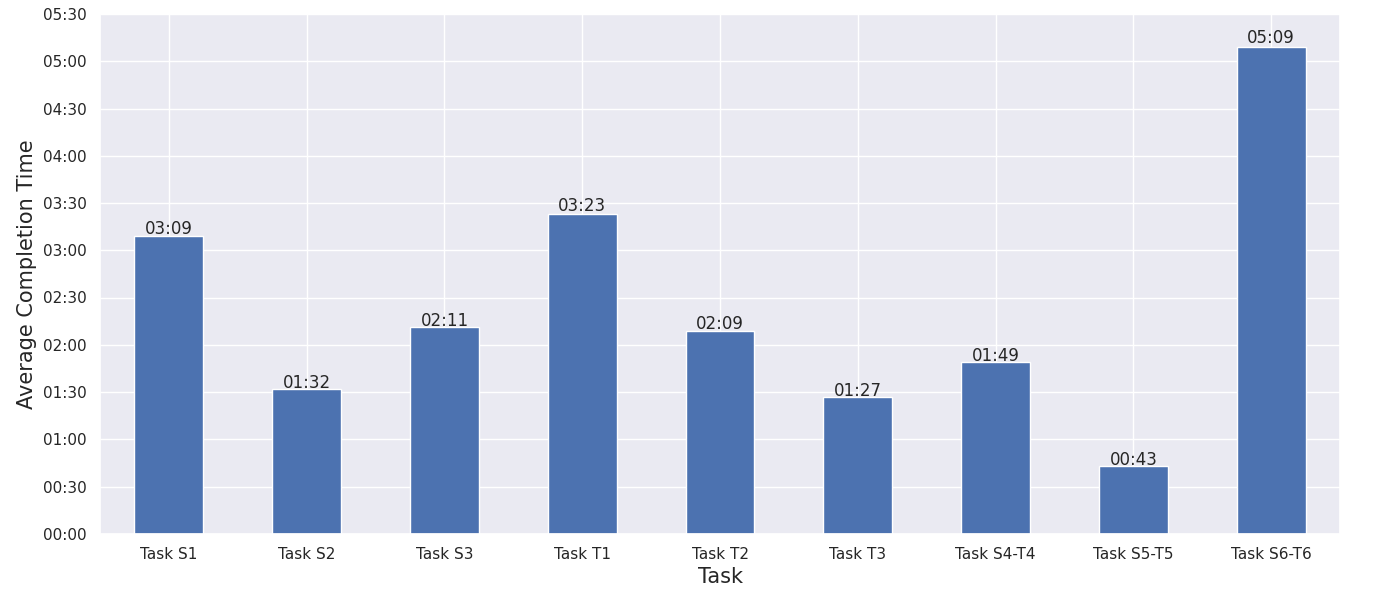
\includegraphics[width=1.1\textwidth]{images/ResultsEfficiencyAvg.png}}%
            \captionsetup{justification=centering}
            \caption{Average completion time for each task}
            \label{ResultsEfficiencyAvg}
        \end{minipage}
    \end{figure}

\pagebreak

\subsubsection{Errors}
    A summary graph in Fig. \ref{BarsErrors} shows the average of user errors for each task.
    \begin{figure}[!ht]
        \begin{minipage}{\linewidth}
            \centering
            \makebox[\textwidth][c]{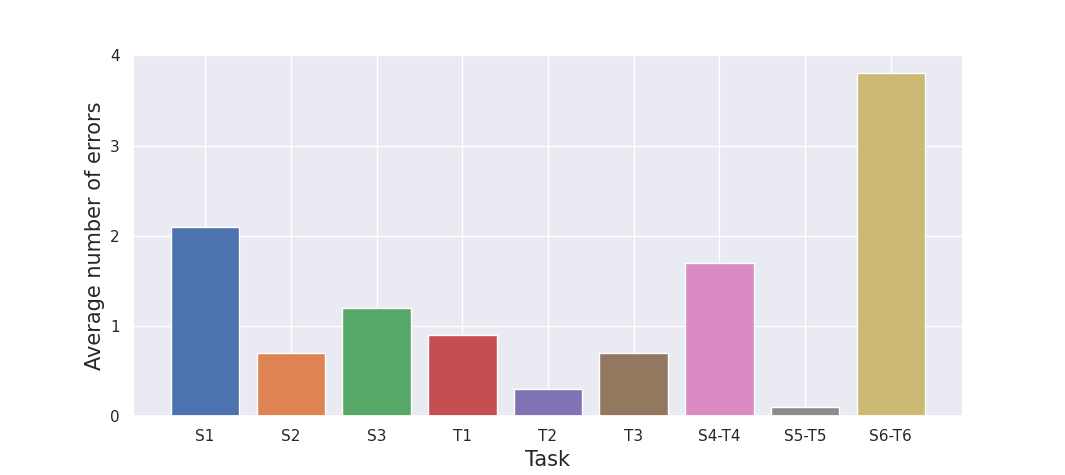
\includegraphics[width=1\textwidth]{images/BarsErrors.png}}%
            \captionsetup{justification=centering}
            \caption{Average of user errors for each task}
            \label{BarsErrors}
        \end{minipage}
    \end{figure}

\subsubsection{Task difficulty}
    A summary graph in Fig. \ref{ResultsDifficulty} shows the difficulty score of each user for each task. The average perceived difficulty is also provided.
    \begin{figure}[!ht]
        \begin{minipage}{\linewidth}
            \centering
            \makebox[\textwidth][c]{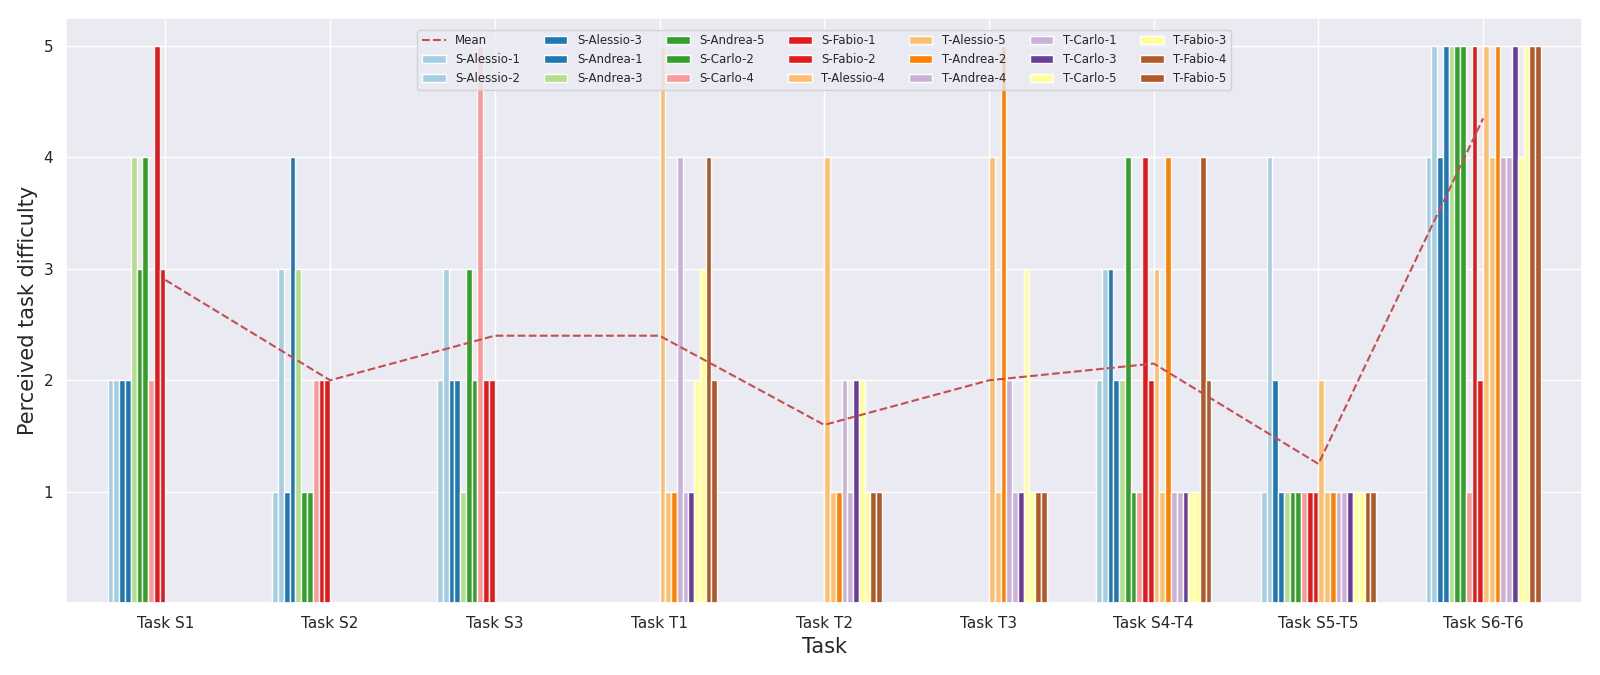
\includegraphics[width=1.3\textwidth]{images/ResultsDifficulty.png}}%
            \captionsetup{justification=centering}
            \caption{Perceived task difficulty of each user and mean}
            \label{ResultsDifficulty}
        \end{minipage}
    \end{figure}


\subsection{Discussion of results}
    % Your observations on results
    % Summary of comments from user testing
    Analyzing the graphs, as expected the users performed poorly on the task S6-T6. The task should not be very difficult, but due to the footer link "all the venues" missing in the main menu it underperformed. As a matter of fact, many it is also the task on which the users spent the most amount of time and committed the most amount of errors.\\
    On the other hand, the task S5-T5 regarding Covid has 100\% completion rate with almost zero errors: a link directly leading to the Covid page is immediately visible on the top of the home page.\\
    Finally, we summarize the various comments of the inspectors in the following points:
    \begin{itemize}
        \item The search bar was used more frequently than we thought so, but it had a negative impact on the user experience. Due to its slowness, many users were left waiting for a long period, wondering if it were a connection problem or not. Some of the users were frustrated and even gave up on the task, while the more patient ones were able to retrieve the queried information and were quite satisfied.
        \item Contrary to what we expected, many users did not notice immediately the main menu on the top right, which leads to confusion and disorientation in the first tasks. In addition, those who knew of its existence preferred to use the search bar.
        \item In many pages there are no searching filters or they're poor (e.g. must-see-attractions page, hotels main page). So the users can't find immediately what they're looking for, resulting in long wandering periods.
        \item Some important links (like "all the venues" mentioned above) are in the footer, so they're rarely seen and used. This leads to wandering periods and disorientation.
        \item The searching form in the restaurant page has some bugs (!!! IN FUTURO dire quali sono questi bug, perchè la pagina è cambiata. !!!). Thus, the website sometimes has an unexpected behavior, causing frustation in the users.
        \item The label "guide to the city" is misleading, in fact many users felt disoriented when they found that it does not lead to information about public transport.
    \end{itemize}
    % !TeX root = ../report.tex

\section{Conclusions}
\subsection{Comparison of results}
Both analyses showed that:\\
- Problem in spatial allocation of important links such as "all the venues", as a matter of fact many users did not find the before mentioned link and failed or partially completed the task S6-T6\\
- The search bar influences the visibility of system status, the page appears to be frozen and many users were frustrated and were waiting for a long time\\

Differences:
- Some users found a number of problems that the inspectors missed during the inspection, we did not expect the search bar so much utilized\\
- Inspectors noticed immediately the main menu\\
- Users ignored the anchor links in pages like "university page" and "renting page"
% Comparison of the results achieved using the 2 methods
% - Problems priority and Suggestions for redesign
% - (Optional: Personal observations on the whole work performed: what did you learn?)
\subsection{Suggestions for redesign}
- Expand the headers of main menu, show the "hamburger menu" only when window is small
- Include "all the venues" in the main menu
- The search bar should be faster
- The link anchors for example in "university page" and "renting" could be put in a side menu
- Improve the filtering method in some pages, for example in "attractions" and in "itineraries" a way to filter according to topics (e.g. art, education...) would be preferable
    \pagebreak
    % !TeX root = ../report.tex

\section{Annex A: Inspection}
% Individual inspectors commented scores (MANDATORY) 
% any relevant information
    \pagebreak
    % !TeX root = ../report.tex

\section{Annex B: User Testing}

\begin{small}

\subsection{Evaluator: Alessio}

\paragraph{User 1 (Student)}
\begin{tabularx}{\linewidth}{c c c c c X}
    \toprule
    \textbf{Task} & \textbf{Success} & \textbf{Time}
     & \textbf{Errors} & \textbf{Difficulty} & \textbf{Comment} \\
    \midrule
    1 & Yes & 2:23 & 2 & 2 & The user reached the events of the year page through a link in the home page, without using the top menu \\ \midrule
    2 & Yes & 0:52 & 1 & 1 & The user used the link to the university page present in the homepage \\ \midrule
    3 & Yes & 2:12 & 1 & 2 & User didn't use the menu \\ \midrule
    4 & Yes & 3:25 & 3 & 2 & The user was disoriented by some labels (guide to the city has no section to public transport section).  The user resorted to the search function in the header. User didn't notice the main menu \\ \midrule
    5 & Yes & 0:49 & 0 & 1 & From the home page it's easy to retrieve this section \\ \midrule
    6 & Partial & 9:47 & 7 & 4 & As stated in the inspection, the page one should visit is very hard to reach. The user decided at one point to use the search function at the top, but as it's very slow, and the user could not understand if it was a network problem or not. After clicking many interactive labels mentioning museums (mainly itineraries related labels) the user asked for help. The hint was to look at the menu/footer, then the user finally found the \emph{All venues} page \\ \bottomrule
\end{tabularx}

\paragraph{User 2 (Student)}
\begin{tabularx}{\linewidth}{c c c c c X}
    \toprule
    \textbf{Task} & \textbf{Success} & \textbf{Time}
     & \textbf{Errors} & \textbf{Difficulty} & \textbf{Comment} \\
    \midrule
    1 & Yes & 1:26 & 2 & 2 & The user found many pages related to \emph{Triennale} through the search functionality, many of which provided no information related to the upcoming event (data, price...) but only a general description of the event and its history, so the user had to visit multiple pages \\ \midrule
    2 & Yes & 1:13 & 0 & 3 & N/A \\ \midrule
    3 & Yes & 2:04 & 0 & 3 & User used the search bar \\ \midrule
    4 & Yes & 1:35 & 2 & 3 & User found confusing labels, \emph{Guide to the city} does not lead to public transport page \\ \midrule
    5 & Yes & 1:45 & 1 & 4 & User was mislead by the \emph{Update COVID-19} label \\ \midrule
    6 & No & 7:55 & 3 & 5 & The user tried multiple times to use the search bar, but gave up due to its slowness \\ \bottomrule
\end{tabularx}

\paragraph{User 3 (Student)}
\begin{tabularx}{\linewidth}{c c c c c X}
    \toprule
    \textbf{Task} & \textbf{Success} & \textbf{Time}
     & \textbf{Errors} & \textbf{Difficulty} & \textbf{Comment} \\
    \midrule
    1 & Partial & 4:04 & 2 & 2 & The user asked for help and the inspector pointed out that there is a search funcionality \\ \midrule
    2 & Yes & 0:57 & 0 & 1 & N/A \\ \midrule
    3 & Yes & 2:01 & 0 & 2 & N/A \\ \midrule
    4 & Yes & 4:19 & 4 & 3 & The user was mislead by \emph{Guide to the city} and did not notice the top menu at first \\ \midrule
    5 & Yes & 1:18 & 0 & 2 & The user took a while to find where and how to take tests, the page anchors were confusing \\ \midrule
    6 & Partial & 6:43 & 4 & 4 & The user found the list of free museums, but asked for help to find the parking information \\ \bottomrule
\end{tabularx}

\paragraph{User 4 (Tourist)}
\begin{tabularx}{\linewidth}{c c c c c X}
    \toprule
    \textbf{Task} & \textbf{Success} & \textbf{Time}
     & \textbf{Errors} & \textbf{Difficulty} & \textbf{Comment} \\
    \midrule
    1 & No & 14:30 & 5 & 5 & The user didn't notice the top menu, so the restaurant page was not reached and the user used the search functionality which lead to no results \\ \midrule
    2 & Yes & 6:10 & 1 & 4 & Due to information overload in the top menu, finding the hotel section required some time \\ \midrule
    3 & Partial & 5:05 & 2 & 4 & The user used the search functionality for a while, then asked if there was a better way to search. The inspector suggested to look for a menu, which the user found in the end. Through the menu finding the itineraries page is easy \\ \midrule
    4 & Yes & 2:51 & 2 & 3 & N/A \\ \midrule
    5 & Yes & 1:00 & 0 & 2 & N/A \\ \midrule
    6 & Yes & 8:13 & 3 & 5 & The user found the list of free museums from the search functionality \\ \bottomrule
\end{tabularx}

\paragraph{User 5 (Tourist)}
\begin{tabularx}{\linewidth}{c c c c c X}
    \toprule
    \textbf{Task} & \textbf{Success} & \textbf{Time}
     & \textbf{Errors} & \textbf{Difficulty} & \textbf{Comment} \\
    \midrule
    1 & Yes & 1:12 & 0 & 1 & N/A \\ \midrule
    2 & Yes & 1:40 & 0 & 1 & N/A \\ \midrule
    3 & Yes & 0:35 & 0 & 1 & N/A \\ \midrule
    4 & Yes & 2:05 & 1 & 1 & N/A \\ \midrule
    5 & Yes & 0:35 & 0 & 1 & N/A \\ \midrule
    6 & No & 11:16 & 6 & 4 & User used search bar but thought they weren't getting results because of its slowness. User overlooked the accessibility section on the attraction page. \\ \bottomrule
\end{tabularx}

\pagebreak

\subsection{Evaluator: Andrea}

\paragraph{User 1 (Student)}
\begin{tabularx}{\linewidth}{c c c c c X}
    \toprule
    \textbf{Task} & \textbf{Success} & \textbf{Time}
     & \textbf{Errors} & \textbf{Difficulty} & \textbf{Comment} \\
    \midrule
    1 & Partial & 00:54 & 1 & 2 & User used the search bar but didn't find the \emph{events of the year} page, instead he found the \emph{events of the month} one. \\ \midrule
    2 & Partial & 02:35 & 3 & 4 & User asked for help and was told to try the menu. Then tried to use the search bar, changed idea because of its slowness and used the browser page search to find the word "economy" (didn't use the links in the university list page). \\ \midrule
    3 & Yes & 01:05 & 1 & 2 & User remebered were the link for students and rent student was. \\ \midrule
    4 & Yes & 00:45 & 1 & 2 & User complained of clicking through too many pages. \\ \midrule
    5 & Yes & 00:08 & 0 & 1 & User found the information remarkably fast. \\ \midrule
    6 & Partial & 02:43 & 8 & 5 & User found a broken link (\href{"Info on museums - art venues open"}{https://www.yesmilano.it/en/see-and-do} and asked for help. Once found the \emph{All venues} page, he was confused by the ``Top'' option. \\ \bottomrule
\end{tabularx}

\paragraph{User 2 (Tourist)}
\begin{tabularx}{\linewidth}{c c c c c X}
    \toprule
    \textbf{Task} & \textbf{Success} & \textbf{Time}
     & \textbf{Errors} & \textbf{Difficulty} & \textbf{Comment} \\
    \midrule
    1 & Yes & 00:57 & 0 & 1 & User found a bug by searching ``porta venezia'' and setting the zone to ``porta venezia'' were no result is displayed \\ \midrule
    2 & Yes & 00:47 & 0 & 1 & User didn't notice the filter option, checked each hotel manually \\ \midrule
    3 & No & 01:17 & 2 & 5 & User gave up \\ \midrule
    4 & Yes & 00:34 & 0 & 4 & User noticed the menu in the top right \\ \midrule
    5 & Yes & 00:07 & 0 & 1 & N/A \\ \midrule
    6 & Yes & 1:57 & 2 & 5 & User gave up before finding the venues list \\  \bottomrule
\end{tabularx}

\paragraph{User 3 (Student)}
\begin{tabularx}{\linewidth}{c c c c c X}
    \toprule
    \textbf{Task} & \textbf{Success} & \textbf{Time}
     & \textbf{Errors} & \textbf{Difficulty} & \textbf{Comment} \\
    \midrule
    1 & Yes & 1:36 & 6 & 4 & User tried \emph{Exhibitions in Milan 2022}, looked for ``triennale'', then noticed the search button and searched for ``triennale'' \\ \midrule
    2 & Yes & 2:05 & 1 & 3 & User managed to find the information through another page [\href{https://www.yesmilano.it/en/articles/programs-and-subjects-offered}{yesmilano.it/en/articles/programs-and-subjects-offered}] \\ \midrule
    3 & Yes & 00:56 & 0 & 1 & N/A \\ \midrule
    4 & Yes & 00:55 & 2 & 2 & N/A \\ \midrule
    5 & Yes & 00:15 & 0 & 1 & N/A \\ \midrule
    6 & No & 1:43 & 4 & 5 & User couldn't find the venues page, tried "Itineraries" instead before asking for help. \\  \bottomrule
\end{tabularx}

\paragraph{User 4 (Tourist)}
\begin{tabularx}{\linewidth}{c c c c c X}
    \toprule
    \textbf{Task} & \textbf{Success} & \textbf{Time}
     & \textbf{Errors} & \textbf{Difficulty} & \textbf{Comment} \\
    \midrule
    1 & Partial & 0:56 & 0 & 4 & User didn't find any result by searching for ``porta venezia'' \\ \midrule
    2 & Partial & 1:54 & 0 & 2 & User got an error message telling them they had been banned from the website. After being told to try with another browser, they found the hotels but didn't notice the filter button. By chance the first hotel they clicked was pet-friendly. \\ \midrule
    3 & Yes & 00:44 & 2 & 2 & Guide to the city > Itineraries > Clicked on "Day Trip" first \\ \midrule
    4 & Yes & 0:31 & 0 & 1 & User found the page through the \emph{Travel Info} section \\ \midrule
    5 & Yes & 0:20 & 0 & 1 & N/A \\ \midrule
    6 & Partial & 03:54 & 3 & 4 & User found a suitable attraction in another way: Must see attractions in Milan > Top 10 Museums you muist visit > 10 free things to do in milan > Civic museums of milan > Palazzo Morando (recalling an information that said it was free). He found the opening times but asked for help to find the parking information \\ \bottomrule
\end{tabularx}

\paragraph{User 5 (Student)}
\begin{tabularx}{\linewidth}{c c c c c X}
    \toprule
    \textbf{Task} & \textbf{Success} & \textbf{Time}
     & \textbf{Errors} & \textbf{Difficulty} & \textbf{Comment} \\
    \midrule
    1 & Yes & 0:34 & 1 & 3 & User scrolled through the most importants events. \\ \midrule
    2 & Yes & 0:53 & 0 & 1 & User found the info throught the menu \\ \midrule
    3 & Yes & 01:10 & 4 & 3 & Used the menu but didn't find the \emph{Study} section immediately. \\ \midrule
    4 & Partial & 01:20 & 3 & 4 & User was confused because they couldn't find a way to the information through the menu \\ \midrule
    5 & Yes & 0:10 & 0 & 1 & N/A \\ \midrule
    6 & Partial & 2:24 & 4 & 5 & User asked for help to find the venues page \\ \bottomrule
\end{tabularx}

\pagebreak

\subsection{Evaluator: Carlo}

\paragraph{User 1 (Tourist)}
\begin{tabularx}{\linewidth}{c c c c c X}
    \toprule
    \textbf{Task} & \textbf{Success} & \textbf{Time}
     & \textbf{Errors} & \textbf{Difficulty} & \textbf{Comment} \\
    \midrule
    1 & Yes & 01:46 & 0 & 1 & The user selected “porta venezia” but the website selected "duomo, centro città" \\ \midrule
    2 & Yes & 01:52 & 0 & 1 & In the hotels.yesmilano page even though the user selected 3 guests (plus dog) the suggestions stated "Perfect for two guests". It's not evident if the price refers to a single night or to the selected period. The selected period doesn't appear \\ \midrule
    3 & Yes & 00:53 & 0 & 1 & Itineraries could implement a search filter \\ \midrule
    4 & Yes & 00:46 & 0 & 1 & The website instead of downloading the map, redirects two times to the ATM website \\ \midrule
    5 & Yes & 01:14 & 0 & 1 & N/A \\ \midrule
    6 & Partial & 03:51 & 1 & 4 & The user doesn't find a way to search for free entrance museums. The user finds a museum with free entrance just by using the search bar, moreover there was only on single result. No information regarding near parking spots is provided. Lack of a filter in the museum section \\ \bottomrule
\end{tabularx}

\paragraph{User 2 (Student)}
\begin{tabularx}{\linewidth}{c c c c c X}
    \toprule
    \textbf{Task} & \textbf{Success} & \textbf{Time}
     & \textbf{Errors} & \textbf{Difficulty} & \textbf{Comment} \\
    \midrule
    1 & Partial & 04:54 & 1 & 4 & The user wasn't able to use the search bar. The user was able to find only a single event based at the triennale. \\ \midrule
    2 & Yes & 01:36 & 0 & 1 & There is the lack of a filtering system in the university page \\ \midrule
    3 & Yes & 3:16 & 1 & 2 & The user missed the rent and housing link. It could be highlighted \\ \midrule
    4 & Yes & 00:35 & 0 & 1 & N/A \\ \midrule
    5 & Yes & 00:40 & 0 & 1 & N/A \\ \midrule
    6 & No & 5:35 & 3 & 5 & The user wasn't able to search for museums with free entrances. After three wrong redirections the task was stopped. \\ \bottomrule
\end{tabularx}

\paragraph{User 3 (Tourist)}
\begin{tabularx}{\linewidth}{c c c c c X}
    \toprule
    \textbf{Task} & \textbf{Success} & \textbf{Time}
     & \textbf{Errors} & \textbf{Difficulty} & \textbf{Comment} \\
    \midrule
    1 & Yes & 00:50 & 0 & 1 & User found no difficulties \\ \midrule
    2 & Partial & 01:50 & 1 & 2 & The user missed the ``pet friendly'' tag \\ \midrule
    3 & Yes & 00:50 & 0 & 1 & N/A \\ \midrule
    4 & Yes & 00:58 & 1 & 1 & The user clicked on a wrong link but immediately realized the mistake. \\ \midrule
    5 & Yes & 01:36 & 0 & 1 & N/A \\ \midrule
    6 & Partial & 03:05 & 2 & 5 & The user was able to find a masterpiece shown in Santa Maria delle Grazie church, which on Sunday can be seen for free. Still, it was a matter of chance \\ \bottomrule
\end{tabularx}

\paragraph{User 4 (Student)}
\begin{tabularx}{\linewidth}{c c c c c X}
    \toprule
    \textbf{Task} & \textbf{Success} & \textbf{Time}
     & \textbf{Errors} & \textbf{Difficulty} & \textbf{Comment} \\
    \midrule
    1 & Yes & 03:23 & 1 & 2 & The user searched "triennale eventi" and noticed the long wait. At the end, the user found the events from the \emph{All the events} filter. Still, he reached the all the events page with some difficulties \\ \midrule
    2 & Yes & 01:12 & 0 & 2 & N/A \\ \midrule
    3 & No & 04:48 & 3 & 5 & By searching ``tenancy'' and ``documents'', the user found no results. After a while the user gave up. \\ \midrule
    4 & Yes & 01:16 & 0 & 1 & N/A \\ \midrule
    5 & Yes & 01:10 & 0 & 1 & The user used the link in the footer. \\ \midrule
    6 & Yes & 03:59 & 0 & 1 & The user noticed that there wasn't a filter for free museum entrance and used the search bar instead and found an useful article. The user noticed that highlighted words might be links. \\ \bottomrule
\end{tabularx}

\paragraph{User 5 (Tourist)}
\begin{tabularx}{\linewidth}{c c c c c X}
    \toprule
    \textbf{Task} & \textbf{Success} & \textbf{Time}
     & \textbf{Errors} & \textbf{Difficulty} & \textbf{Comment} \\
    \midrule
    1 & Yes & 01:56 & 0 & 2 & The page for booking a restaurant resetted user inputs multiple times. \\ \midrule
    2 & Yes & 02:20 & 0 & 2 & N/A \\ \midrule
    3 & Yes & 02:55 & 1 & 3 & N/A \\ \midrule
    4 & Yes & 01:24 & 0 & 1 & N/A \\ \midrule
    5 & Yes & 00:20 & 0 & 1 & N/A \\ \midrule
    6 & Yes & 02:30 & 0 & 4 & The user found a useful article by chance. \\  \bottomrule
\end{tabularx}

\pagebreak

\subsection{Evaluator: Fabio}

\paragraph{User 1 (Student)}
\begin{tabularx}{\linewidth}{c c c c c X}
    \toprule
    \textbf{Task} & \textbf{Success} & \textbf{Time}
     & \textbf{Errors} & \textbf{Difficulty} & \textbf{Comment} \\
    \midrule
    1 & No & 8:00 & 3 & 5 & The user tried to use to search bar (both the one at the top of the page and the one specific for events) with no success. Then she tried to look at the events of the different months with no success. \\ \midrule
    2 & Yes & 2:37 & 1 & 2 & The user first tried the \emph{Study} page (reached from homepage), then went on the \emph{Rent} page. \\ \midrule
    3 & Partial & 2:30 & 1 & 2 & The user wasn't sure if they reached the right page, then after a hint she found the solution. \\ \midrule
    4 & Yes & 3:20 & 2 & 4 & The user found difficulties at the beginning because she didn't use the menu at the top-right of the page, and said that such information should be in the homepage \\ \midrule
    5 & Yes & 0:33 & 0 & 1 & N/A \\ \midrule
    6 & No & 9:09 & 5 & 5 & Event after various hints, the user didn't find the solution. \\ \bottomrule
\end{tabularx}

\paragraph{User 2 (Student)}
\begin{tabularx}{\linewidth}{c c c c c X}
    \toprule
    \textbf{Task} & \textbf{Success} & \textbf{Time}
     & \textbf{Errors} & \textbf{Difficulty} & \textbf{Comment} \\
    \midrule
    1 & Yes & 4:25 & 2 & 3 & The user didn't use the top-right menu. Then, he found the solution by using the search on the bar at the top of the homepage \\ \midrule
    2 & Yes & 1:25 & 1 & 2 & Searching for "university" yielded no result, then he found the top-right menu. \\ \midrule
    3 & Yes & 1:55 & 1 & 2 & User clicked on ``moving to Milano'', instead of ``living in Milano'' [\href{https://www.yesmilano.it/en/welcome-to-milano}{https://www.yesmilano.it/en/welcome-to-milano}]. \\ \midrule
    4 & Yes & 0:49 & 0 & 2 & N/A \\ \midrule
    5 & Yes & 0:30 & 0 & 1 & N/A \\ \midrule
    6 & No & 1:40 & 0 & 2 & The user mistakenly thought he reached the right page. They used the search bar to find ``free museums'' and clicked on the result ``10 free things to do in Milan'', and found a free museum by chance. They found the opening hours and how to reach it \\ \bottomrule
\end{tabularx}

\paragraph{User 3 (Tourist)}
\begin{tabularx}{\linewidth}{c c c c c X}
    \toprule
    \textbf{Task} & \textbf{Success} & \textbf{Time}
     & \textbf{Errors} & \textbf{Difficulty} & \textbf{Comment} \\
    \midrule
    1 & Yes & 2:16 & 1 & 3 & The user had problems finding the Restaurants section of the webiste \\ \midrule
    2 & Yes & 1:07 & 0 & 1 & The user completed this task quickly thanks to the previous experience with YesMilano restaurants \\ \midrule
    3 & Yes & 0:30 & 0 & 1 & N/A \\ \midrule
    4 & Yes & 0:34 & 0 & 1 & N/A \\ \midrule
    5 & Yes & 0:23 & 0 & 1 & N/A \\ \midrule
    6 & Partial & 5:33 & 3 & 5 & The initial navigation flow was: ``Menu > Attrazioni > 10 musei da non perdere'' \\ \bottomrule
\end{tabularx}

\paragraph{User 4 (Tourist)}
\begin{tabularx}{\linewidth}{c c c c c X}
    \toprule
    \textbf{Task} & \textbf{Success} & \textbf{Time}
     & \textbf{Errors} & \textbf{Difficulty} & \textbf{Comment} \\
    \midrule
    1 & Partial & 5:00 & 2 & 4 & The user used multiple times the top search bar with no success. Only after an hint he used the menu at the top right. \\ \midrule
    2 & Yes & 2:12 & 1 & 1 & At the beginning the user clicked on ``Weekend Milano'' in the homepage, but then he used the top right menu.  \\ \midrule
    3 & Yes & 0:50 & 0 & 1 & Top-right menu > Itineraries > What to see in Milan in 3 days \\ \midrule
    4 & Yes & 4:35 & 3 & 4 & The user first clicked "Guida alla città" on the homepage, then he clicked on ``Itineraries'' and then on ``Attractions'' (both are in the top right menu), then he found the correct link \\ \midrule
    5 & Yes & 0:20 & 0 & 1 & On the homepage he clicked "Vivi la città in sicurezza" \\ \midrule
    6 & Partial & 7:20 & 3 & 5 & After many navigation errors, the user found the ``All venues'' link in the footer. \\ \bottomrule
\end{tabularx}

\paragraph{User 5 (Tourist)}
\begin{tabularx}{\linewidth}{c c c c c X}
    \toprule
    \textbf{Task} & \textbf{Success} & \textbf{Time}
     & \textbf{Errors} & \textbf{Difficulty} & \textbf{Comment} \\
    \midrule
    1 & Yes & 4:33 & 1 & 2 & The user mistakenly he clicked on "Weekend a Milano" in the homepage \\ \midrule
    2 & Yes & 1:42 & 0 & 1 & N/A \\ \midrule
    3 & Yes & 0:58 & 0 & 1 & N/A \\ \midrule
    4 & Yes & 1:17 & 1 & 2 & The user first clicked "Guida alla città" on the homepage. \\ \midrule
    5 & Yes & 0:45 & 0 & 1 & N/A \\ \midrule
    6 & No & 9:12 & 4 & 5 & Despite an hint, the user did not find the solution \\ \bottomrule
\end{tabularx}

\end{small}

\end{document}